\documentclass[12pt]{article}
% Load packages
\usepackage{url}  % Formatting web addresses
\usepackage{ifthen}  % Conditional
\usepackage{multicol}   %Columns
\usepackage[utf8]{inputenc} %unicode support
\usepackage{amsmath}
\usepackage{amssymb}
\usepackage{epsfig}
\usepackage{epstopdf}
\usepackage{graphicx}
\usepackage[margin=0.1pt,font=footnotesize,labelfont=bf]{caption}
\usepackage{setspace}
%\usepackage{longtable}
\usepackage{colortbl}
%\usepackage{palatino,lettrine}
%\usepackage{times}
%\usepackage[applemac]{inputenc} %applemac support if unicode package fails
%\usepackage[latin1]{inputenc} %UNIX support if unicode package fails
\usepackage[wide]{sidecap}
%\usepackage[authoryear,round,comma,sort&compress]{natbib}
\usepackage[square,sort,comma,numbers,sort&compress]{natbib}
%\usepackage[authoryear,round]{natbib}
\usepackage{supertabular}
\usepackage{simplemargins}
\usepackage{fullpage}
\usepackage{comment}
\usepackage{lineno}
%\usepackage{chicago}
\usepackage{textcomp}
\usepackage{multirow}
\usepackage{amsmath}
\usepackage[linesnumbered,lined,boxed,commentsnumbered]{algorithm2e}
\DeclareMathOperator*{\argmin}{\arg\!\min}

\usepackage{algorithm2e}
\usepackage{algpseudocode}
%\usepackage[space]{cite}
\urlstyle{rm}

%\textwidth = 6.50 in
%\textheight = 9.5 in
%\oddsidemargin =  0.0 in
%\evensidemargin = 0.0 in
%\topmargin = -0.50 in
%\headheight = 0.0 in
%\headsep = 0.25 in
%\parskip = 0.15in
%\linespread{1.75}
\doublespace

%\bibliographystyle{chicago}
\bibliographystyle{plos2009}

\makeatletter
\renewcommand\subsection{\@startsection
	{subsection}{2}{0mm}
	{-0.05in}
	{-0.5\baselineskip}
	{\normalfont\normalsize\bfseries}}
\renewcommand\subsubsection{\@startsection
	{subsubsection}{2}{0mm}
	{-0.05in}
	{-0.5\baselineskip}
	{\normalfont\normalsize\itshape}}
\renewcommand\section{\@startsection
	{subsection}{2}{0mm}
	{-0.2in}
	{0.05\baselineskip}
	{\normalfont\large\bfseries}}
\renewcommand\paragraph{\@startsection
	{paragraph}{2}{0mm}
	{-0.05in}
	{-0.5\baselineskip}
	{\normalfont\normalsize\itshape}}
\makeatother

%Review style settings
%\newenvironment{bmcformat}{\begin{raggedright}\baselineskip20pt\sloppy\setboolean{publ}{false}}{\end{raggedright}\baselineskip20pt\sloppy}

%Publication style settings

% Single space'd bib -
\setlength\bibsep{0pt}

\renewcommand{\rmdefault}{phv}\renewcommand{\sfdefault}{phv}
\newcommand{\norm}[1]{\left\lVert#1\right\rVert}

% Change the number format in the ref list -
\renewcommand{\bibnumfmt}[1]{#1.}

% Change Figure to Fig.
\renewcommand{\figurename}{Fig.}

% Begin ...
\begin{document}
\begin{titlepage}
{\par\centering\textbf{\Large {Reduced order modeling and analysis of the human complement subsystem}}}
\vspace{0.05in}
{\par \centering \large{Adithya Sagar, Wei Dai$^{\#}$, Mason Minot$^{\#}$, and Jeffrey D. Varner$^{*}$}}
\vspace{0.10in}
{\par \centering {School of Chemical and Biomolecular Engineering}}
{\par \centering {Cornell University, Ithaca NY 14853}}
\vspace{0.1in}
{\par \centering \textbf{Running Title:}~Reduced order model of complement}
\vspace{0.1in}
{\par \centering \textbf{To be submitted:}~\emph{PLoS~ONE}}
\vspace{0.5in}
{\par \centering $^{\#}$ Denotes equal contribution}
\vspace{0.1in}
{\par \centering $^{*}$Corresponding author:}
{\par \centering Jeffrey D. Varner,}
{\par \centering Professor, School of Chemical and Biomolecular Engineering,}
{\par \centering 244 Olin Hall, Cornell University, Ithaca NY, 14853}
{\par \centering Email: jdv27@cornell.edu}
{\par \centering Phone: (607) 255 - 4258}
{\par \centering Fax: (607) 255 - 9166}
\end{titlepage}
\date{}
\thispagestyle{empty}
\pagebreak
%%%%%%%%%%%%%%%%%%%%%%%%%%%%%%%%%%%%%%%%%%%%%%%%%%%%%%%%%%%%%%%%%%%%%%%%%%%%%%%%%%%%%%%%%%%%%%%%%%%%%%%%%%%
%%%%%%%%%%%%%%%%%%%%%%%%%%%%%%%%%%%%%%%%%%%%%%%%%%%%%%%%%%%%%%%%%%%%%%%%%%%%%%%%%%%%%%%%%%%%%%%%%%%%%%%%%%%
\section*{Abstract}
Complement is a central part of innate immunity and plays a significant role in regulating the inflammatory response. In this study, we build a reduced order model of complement to study the human complement system.
The key novelty of our approach is the use of Ordinary Differential Equations (ODEs) along with logical rules to capture the behavior of a complex biochemical network.  Using this framework we constructed a model of complement that analyzed the dynamics of C3a and C5a when initiated through the alternate and lectin pathways. The reduced order model consisted of only 18 differential equations with 28 kinetic and control parameters. Thus, the model was an order of magnitude smaller that any existing model of complement that includes alternate and lectin pathways. 


%and includes more pathways than comparable purely ODE models in the literature. We estimated the model parameters from in vitro human complement time-course experiments of C3a and C5a from Morad and coworkers, in the presence and absence of zymosan, and without the classical pathway. 

%We then compared the model predictions with C3a and C5a data sets, for alternative and lectin pathway dynamics, that were not used for model training. Once validated, we performed sensitivity analysis on the model to estimate which parameters were critical to model performance in several conditions. The reduced order hybrid approach produced a surprisingly predictive human complement model, much similar to the study on human coagulation using the same modeling framework \cite{sagar2015dynamic}. Taken together, the combined analysis of alternate and lectin pathways along with the incorporation of the downstream reactions involving C5 convertase elucidated new insight into roles of governing parameters that mediate the complement system. Deeply understanding how the main governing parameters change with respective to the different combinations of pathway activation will greatly aid in development of drugs for strategic therapeutic targets. Due to the low computational cost relative to the existing models and accuracy of our predictions, we believe that our reduced order complement network is the first step towards building a computation toolbox for treatment analysis or clinical screening in the medical field.


\vspace{0.1in}
{\noindent \textbf{Keywords:}~Biochemical engineering, systems biology, reduced order models, complement system}

\pagebreak

\setcounter{page}{1}

% Uncomment in production -
\linenumbers


\section*{Introduction}
Complement is a central part of innate immunity and plays a very significant role in regulating the inflammatory response. It was first discovered in the 1890s where it was found to 'complement' the bactericidal activity of natural antibodies. Complement is mediated through a set of approximately 30-35 soluble and cell surface proteases \cite{}. The central process in complement activation involves the formation of Membrane Attack Complex (MAC) and a protein called C5a. Complement activation takes places through three different pathways: the alternate, the classical and the lectin. Each of these pathways involves a different initiator signal that leads to the formation of a serine protease called C5 convertase which cleaves an inactive protein called C5 to form C5a and C5b. The classical pathway is triggered when antibodies form complexes with foreign antigens or other pathogens. A multimeric protein complex C1 binds to the antigen-antibody complex and undergoes a conformational change. This activated complex cleaves proteins C4 and C2 to C4a, C4b, C2a and C2b respectively. C4a and C2b combine to form a protease C4bC2a also known as the classical C3 convertase. The lectin pathway is initiated through the binding of L-ficolin or Mannose Binding Lectin (MBL) to the carbohydrates on the surfaces of bacterial pathogens. This bound complex in turn cleaves C4 and C2 and leads to the production of C4bC2a. The alternate pathway involves a 'tickover' mechanism in which a protein called C3 is hydrolyzed to form C3b. In presence of foreign pathogens C3b binds to these surfaces and recruits  additional factors called factor B and factor D that lead to the formation of alternate C3 convertase - C3bBb. The formation of classical and alternate C3 convertases on bacterial surfaces is followed by the formation of proteases called C5 convertases. The classical and alternate C3 convertases recruit C3, Factor B and Factor D to form classical C5 convertase (C4bC2aC3b) and alternate C5 convertase (C3bBbc3B) respectively. The C5 convertases then cleave C5 to form C5a and C5b respectively. 	The cleavage of C5 is followed by a series of sequential cleavages of proteins C6, C7, C8 and C9 that combine with C5b to form the MAC complex. The activation of complement and formation of C5a and MAC complex is regulated at different points through a number of plasma and host cell proteins. The initiation of the classical pathway through the attachment of C1 to an antibody is controlled by the C1 Inhibitor (C1-Inh), a protease inhibitor belonging to the serpin superfamily. C1-Inh irreversibly binds to and deactivates the active subunits of component C1 to prevent spontaneous fluid phase and chronic activation of complement \cite{walker1995complement}. The serum and host-tissue regulation of the upstream elements of the complement system is also achieved through the binding of C4 binding protein (C4BP) to C4b and through the binding of factor H to C3b \cite{blom2001structural}. These proteins are also capable of binding their respective components in the convertase form. Membrane cofactor protein (MCP or CD46) possesses a cofactor activity for C4b and C3b, which protects the host from self-activation of complement \cite{riley2004cd46}.  Decay accelerating factor (DAF or CD55) is able to recognize and dissociate both convertases \cite{lukacik2004complement}. MAC is inhibited by vitronectin and clusterin in the plasma and CD59 at the host surface.
Proteins C3a, C4a, and C5a are inactivated or reduced in activity by carboxypeptidase-N \cite{liszewski1995control}. Research over the past decade has also shown that the role of complement extends beyond as a simple player in the immune system. It is an important network in maintaining homeostasis and malfunction of complement has been linked with several diseases like Alzheimers, acute macular degeneration (AMD), glaucoma, Parkinson's disease, multiple sclerosis, renal failure, schizophrenia, rheumatoid arthritis, cancer, sepsis and coagulopathy. The ability to maintain cross talk with other networks like coagulation, autonomous nervous response and the ability to regulate inflammation makes it important to understand complement in a more holistic perspective. 

Thus given the complexity and importance of complement in influencing the human condition, developing models of complement within an integrative framework (that includes other biochemical networks) are crucial to understanding its role in human disease. Traditionally, complement models have been formulated as linear or non-linear Ordinary Differential Equation (ODE) systems. Hirayama  et al. (ref) used a system of linear ODEs to model the classical pathway of complement. Korotaevskiy and co-workers (ref) built a theoretical model of complement using a system of non-linear ODEs that included classical, lectin and alternate pathways. However both these studies involve no validation studies with experimental data. Liu et al analyzed the formation of classical and lectin C3 convertases and the regulatory role of C4BP using a system of 45 non-linear ODEs with 85 parameters.  Recently, Zewde and co-workers built a detailed mechanistic model of alternative complement activation was built using 107 ODEs and 74 kinetic parameters (Ref). This model delineated the response of complement on a host cell and a foreign antigen. However, these previous models were largely based upon mechanistic knowledge.  Given the complexity of complement and its interactions with other networks it is unfeasible and computationally expensive to build such large mechanistic models. In addition is much more difficult to experimentally interrogate the response of various complement proteins under different conditions. This also presents with the problem of estimation of a large number of parameters with little or no experimental data. Thus there exists a need to reduce the mechanistic complexity while capturing dynamics of complement accurately.

In this study, we present a hybrid modeling approach to build a reduced order model of complement. The key innovation of this approach is the use of simple equations to capture the behavior of a complex biochemical network. The hybrid approach combines ODEs with logical rules to model biochemical processes that are complex or for which a complete mechanistic understanding is missing. We used this framework to capture dynamics of C3a and C5a formation in the lectin and alternative pathways. The reduced order model consisted of only 18 differential equations with 28 kinetic and control parameters. Thus, the model was an order  of magnitude smaller and included more pathways than comparable ODE models in the literature. We estimated the model parameters from in vitro time series data of C3a and C5a from Morad and coworkers \cite{morad2015time}. Subsequently we validated the model on unseen C3a and C5a experimental data that were not used for model training.  After validation, we performed a sensitivity analysis on the model to estimate which parameters were critical to model performance under different experimental conditions. Given its small size, the hybrid approach produced a surprisingly predictive human complement model, similar to an earlier study on human coagulation using the same modeling framework \cite{sagar2015dynamic}. Taken together, the combined analysis of alternate and lectin pathways along with the incorporation of the downstream reactions involving C5 convertase elucidated new insight into the roles of parameters that govern the complement system.  A deeper understanding about how these parameters influence complement dynamics will greatly aid in the development of drugs for strategic therapeutic targets. Due to the low computational cost relative to the existing models and accuracy of our predictions, we believe that our reduced order complement network is the first step towards building a computation toolbox for screening drug potential drug targets or therapeutic agents that can be targeted against complement.
\clearpage

\section*{Results}

\subsection*{Formulation of a reduced order complement model}
We developed a reduced order human complement network consisting of the most crucial steps of the human complement system (Fig. \ref{fig-schematic}). The core of our model was based upon the experimental measurements of Morad and coworker's earlier work \cite{morad2015time}, we only consider the activation of complement system through the alternate and the lectin pathways. In doing so we aim to capture a complex biological phenomenon using a few simple ordinary differential equations.  A trigger event initiates the lectin pathway in the presence of zymosan, which activates the cleavage of C2 and C4 into C2a and C2b, and C4a and C4b respectively. Classical Pathway (CP) C3 convertase (C4aC2b) is a combination of C4a and C2b, which catalyzes the cleavage of C3 into C3a and C3b. Similarly, the activation of the alternative pathways happens through the spontaneous hydrolysis of C3 which facilitates the cleavage of C3. C3b then could combine with with C3 to form alternate pathway (AP) C3 convertase. Both C3 convertases catalyze the cleavage of C3 into C3a and C3b, and C3b can then combine with either CP or AP C3 convertase to form C5 convertase, CP or AP respectively that is responsible for the cleavage of C5 to C5a and C5b. Lectin pathway activation was approximated using a combination of saturation kinetics and Hill-like function control functions. These control coefficients then modified the rates of model processes at each time step. Hill-like transfer functions $0 \le \mathbf{f (Z)}  \le 1$ quantified the contribution of components upon a target process, in this study, $\mathbf{Z}$ represents the abundance of the initiator. Taken together, while the reduced order human complement model encodes significant biological complexity, it is highly compact (consisting of only 18 differential equations). Thus, it will serve as an excellent proof of principle example to study the reduction of a highly complex human subsystem.

\subsection*{An ensemble of complement models was estimated using dynamically dimensioned search.}
A critical challenge for any dynamic model is the estimation of kinetic parameters. We estimated
kinetic and control parameters in a hierarchical fashion using  two $in~vitro$ time-series human complement data sets with and without zymosan present. The residual between simulation and experimental measurements were minimized  using dynamically dimensioned search (DDS). An initial parameter set was initialized with randomized kinetic and control parameters and allowed to search for parameter vectors that minimized the residual. Knowing that the kinetic and control parameters of the lectin pathway does not affect the dynamics of the alternate pathway, we used a hierarchal approach that estimated the parameters for the alternative pathway and lectin pathway separately. For the alternative pathway, we utilized the time-course experimental measurements of Morad and coworkers \cite{morad2015time} of C3a and C5a in the absence of zymosan and only allowed the alternative parameters to vary (Fig. \ref{fig-fit} A and B). The estimated alternate parameters was then fixed for the determination of lectin pathway parameters. The training for the lectin parameters, we used the experimental measurements of C3a and C5a in the presence of $1$ g of zymosan published by Morad et al \cite{morad2015time} (Fig. \ref{fig-fit} C and D).
The reduced human complement model captured the behavior of the alternative and lectin pathways through the time-course abundance of C3a and C5a (Fig. \ref{fig-fit}).
However we were not able to capture the curvature of the C5a alternative (Fig. \ref{fig-fit}).
The decreasing slope of the experimental measurements may be an indication of the decreasing cofactors that are required for the spontaneous hydrolysis in the alternative pathway, which we neglected.  Taken together, the model identification results suggested that our reduced order approach could reproduce a panel of lectin pathway initiation data sets in the neighborhood of physiological factor and inhibitor concentrations. However, it was unclear whether the reduced order model could predict new data, without updating the model parameters.

We tested the predictive power of the reduced order human complement model with validation data sets not used during model training. Six validation data sets were used, three for C3a and C5a respectively at different zymosan concentrations. All kinetic and control parameters were
fixed for the validation simulations. The reduced order model predicted the C3a and C5a time-course profiles at a qualitative level (Fig. \ref{fig-prediction}). [AND THEN WHAT??]

\subsection*{Global Sensitivity analysis of the reduced order complement model}
We conducted a Sobol's sensitivity analysis to estimate which parameters controlled the performance of the reduced order model. We calculated the sensitivity of the change in C3a and C5a profiles using the residuals between simulation and experimentally measured data for the cases of 0 and 1g zymosan (Fig. \ref{fig-SA}.
For the cases in absence of zymosan where only the alternative pathway is active, we observed that only a few variables are responsible for the system response. For C3a alternate, the sensitivity analysis found that $k_{c3b~basal}$ and $k_{degradationC3a}$ are the only sensitive parameters. This gives us new insight in which of the parameters play a role in complement activation. Even though AP~C3~convertase is also responsible in the conversion of C3 and the production of C3a, the kinetic parameters that govern the equation was not sensitive at all. This elucidated that the activation of alternative pathway is more heavily governed by the spontaneous hydrolysis of C3 rather than the activity of AP~C3~Convertase. Surprisingly, closely examining the sensitive parameters that control C5a, in addition to the expected kinetic and control parameters related to the formation of AP~C5~Convertase, we observed that $k_C3~Convertase2$, the was previously not sensitive to C3a, to be sensitive in the formation of C5a. The AP~C3~Convertase is a substrate required for the formation of AP~C5~Convertase and the formation of C3b. The change in activity of AP C3 Convertase  will not drastically change the C3a dynamics, but will effect AP~C5a~Convertase formation and C5a formation.
The our reduced order human complement model in combination with Sobol's sensitivity analysis was able to unravel important indirect parameter interaction.
Our sensitivity analysis yielded expected results for the lectin pathway analyzes (Fig. \ref{fig-SA} (C and D)). One key difference that was observed between the sensitivity of the parameters between C3a an C5a was their respective degradation terms. The degradation constant of C3a was sensitive between the two different cases of zymosan that was tested while the degradation constant of the C5a was not sensitive. We believe this different is attributed to the magnitude of the parameters and their respective concentrations.

\clearpage

%As the dimensionality of  increases, the search region gets widened and thus the problem becomes more challenging.
%

\section*{Discussion}

The discussion has three (sometimes four) paragraphs:
\begin{enumerate}
	\item{\textbf{First~paragraph}: Present a modified version of the last paragraph of the introduction. In this study, [...]. Taken together, [killer statement]}
	
	In this study, we present a hybrid modeling approach to build a reduced order model of complement. The key innovation of this approach is the use of simple equations to capture the behavior of a complex biochemical network. The hybrid approach combines ODEs with logical rules to model biochemical processes that are complex or for which a complete mechanistic understanding is missing. We used this framework to capture dynamics of C3a and C5a formation in the lectin and alternative pathways. The reduced order model consisted of only 18 differential equations with 28 kinetic and control parameters. Thus, the model was an order  of magnitude smaller and included more pathways than comparable ODE models in the literature. We estimated the model parameters from in vitro time series data of C3a and C5a from Morad and coworkers \cite{morad2015time}. Subsequently we validated the model on unseen C3a and C5a experimental data that were not used for model training.  After validation, we performed a sensitivity analysis on the model to estimate which parameters were critical to model performance under different experimental conditions. Given its small size, the hybrid approach produced a surprisingly predictive human complement model, similar to an earlier study on human coagulation using the same modeling framework \cite{sagar2015dynamic}. Taken together, the combined analysis of alternate and lectin pathways along with the incorporation of the downstream reactions involving C5 convertase elucidated new insight into the roles of parameters that govern the complement system.  A deeper understanding about how these parameters influence complement dynamics will greatly aid in the development of drugs for strategic therapeutic targets. Due to the low computational cost relative to the existing models and accuracy of our predictions, we believe that our reduced order complement network is the first step towards building a computation toolbox for screening drug potential drug targets or therapeutic agents that can be targeted against complement.

	\item{\textbf{Second~paragraph}: Contrast the key findings of the study with other computational/experimental studies}
	
Though the role of complement in immune response has been well known since long, there has been a paucity of mathematical models of complement. To our knowledge this is the first model of complement that combines different pathways of initiation and validates the dynamics of downstream proteins like C5a using experimental data. Liu and co-workers modeled formation of C3a through the classical pathway using 45 non-linear ODEs  \cite{liu2011computational}. The hybrid modeling framework, however, allowed us to model the lectin mediated formation of C3a using only 5 ODEs.  Though we do not model all the interactions of initiation in detail, especially the cross-talk between lectin and classical pathways like Liu et al. \cite{liu2011computational} we successfully captured C3a dynamics with respect to different concentrations of lectin initiators. The model was also surprisingly accurate in capturing the quantitative dynamics of C3a and C5a formed from the alternate pathway with only 7 ODEs. The lag phase in the initiation of C5a is followed by an acceleration in the production of C5a. This is also qualitatively similar to the predicted C5a time profiles using a theoretical model of complement with 107 equations \cite{zewde2016quantitative}. Similarly, our model was able to capture C3a formation from the alternate pathway that showed the same qualitative trends as Zewde et al \cite{zewde2016quantitative}. We also observe in our model simulation that the quantity of C3a produced in the alternate pathway is nearly 1000 times the quantity of  C5a produced. Though this is in agreement with the experimental data  \cite{morad2015time}, it differs from the theoretical predictions by Zewde et al.\cite{zewde2016quantitative} who show that C3a is ${10^8}$ times the C5a concentration. It is possible that the experimental system has trace amounts of C5a which leads to this difference. In our model the time profile of C5a generation from the lectin pathway changes with respect to the quantity of zymosan (the lectin pathway initiator). We see that the lag phase for generation progressively decreases with increasing concentration of the initiator. Korotaevskiy et al. \cite{korotaevskiy2009non} show a similar lag phase followed by an accelerated production of C5a using a theoretical model of complement for much smaller time scales. Zewde et al. \cite{zewde2016quantitative} show a similar time profile for C5a generated in the alternate pathway as well. We do observe a similar trend in our model. However given the different time scale in our study we do not observe a very prominent lag phase. Our model also captures the maximum concentrations of C5a with different initiators and in the alternate pathway. However we do not capture the maximum concentration of C3a with low initiator levels though we capture the overall trend which includes the initiation and amplification phases. One of the possible reasons for this could be the non-inclusion of C2-by pass pathway which further accelerates production of C3a without the involvement of a C3 convertase. Currently the C3a in the model is generated only through the activity of a C3 convertase. Incorporating this additional step within the reduced order modeling framework would be a future direction that we need to consider. Taken together we surprisingly do very well in capturing the dynamics of key complement proteins and observe similar trends as in large mechanistic models.

%%% We talk about complement therapeutics here in relation with sensitivity analysis

The global sensitivity analysis of our reduced order model provides interesting insights into the regulation of C3a and C5a which are important therapeutic targets.  We see that the formation of C5a in the absence of an initiator is the most sensitive to the formation of basal C3b through the tick over mechanism. This mechanism could be a potential target for C5a inhibitors especially in cases of autoimmune disorders where there is an absence of initiators of the lectin or the classical pathway. In presence of an initiator we see that C5a formation is primarily sensitive to the lectin initiation parameters and the kinetic parameters that govern the conversion of C5 to C5a and C5b. This result agrees well with the current protease inhibitors targeting initiating complexes that includes mannose-associated serine proteases 1 and  2 (MASP-1,2). The most commonly used anti-complement drug eculizumab, targets C5 protein which is cleaved to form C5a. Our sensitivity analysis shows that kinetic parameters governing C5 conversion are sensitive in both lectin initiated and alternate pathways, thus agreeing with targeting C5 protein. The formation of basal C3b is also a sensitive parameter in the formation of C3a through the alternate pathway. Thus this mechanism can act as a target for both C3a and C5a inhibitors. The lectin initiated formation of C3a shows a number of sensitive parameters. This includes the lectin initiation parameters that control the formation of C5a along with C3 convertase inhibition using C4BP and the parameter governing C3 convertase. All these mechanisms involve potential drug targets and literature shows that C4BP, C3 convertase inhibitors are the being developed as the next generation inhibitors of complement \cite{morgan2015complement}. Taken together it is surprising to see that reduced order model has the ability to identify mechanisms for potential drug targets that are in agreement with existing literature.
%Though it is known complement malfunction causes a number of diseases \cite{ricklin2007complement} developing complement specific therapeutics has been challenging\cite{ricklin2007complement}. Currently there are only four approved drugs targeting complement \cite{morgan2015complement}. Eculizumab targets C5, Berinert, Ruconest and Cinryze target C1. 
 
	\item{\textbf{Third~paragraph}: Present future directions. If you had more time, what would like to do? Highlight the key shortcomings of the approach and how will we address them in the future.
	In this case, we will have a scaling issue if we extend to genome scale. We should extend to dynamic cases, and we need to experimentally validate the findings. }
\end{enumerate}
%This suggests that our reduced order model's prediction for the alternate pathway have great potential application for the study of glomerular diseases that show strong correlation with disturbed alternative pathway activity (Pickering2011). In the diseases driven by dysfunctional alternative pathway, the activation of C5 appears to be the source that fueled the cycle by causing endothelial damage. 

The performance of the reduced order complement model was impressive given its limited size. However, there are several critical questions that should be explored following this study. A logical progression for this work would include expanding the network to include the classical pathway and the formation of the membrane attack complex (MAC). It is unclear whether the addition of the classical pathway will decrease the prediction of our existing model due to the cross-talk between the classical and lectin activation shown by Liu et al \cite{liu2011computational}. One potential approach in addressing such difficulties would be the incorporation of additional species such as C reactive proteins (CRP) and L-ficolin (LF) that involved in complement initiation of classical and lectin pathways. The influence of CRP, LF and the cross-talk can be captured through additional control functions that act upon the initiation pathways in a logical integration rule developed by Wayman and coworkers \cite{wayman2015dynamic}. Another issue with our reduced order model involve the omitted species that are implicitly lumped together with our effective kinetics and control parameters. Due to the reduction of parameters, the model cannot determine the dynamics or explicit impact of the omitted species on the system. However, we have created a hierarchy approach for parameter estimation that can be used to uncouple the kinetic parameter and contribution of any additional complement proteins and regulators. Using this simple and versatile modeling approach that we created, we took the first step in the development of a computation toolkit that can be readily used in a clinical setting. Our reduced order complement model is computationally inexpensive, and versatile so it could easily be incorporated into pre-existing or new pharmacokinetic models. Furthermore this approach model has the potential to create individualized treatment plans for patients with complement deficiency.

\clearpage

\section*{Materials and Methods}
We used ordinary differential equations (ODEs) to model the time evolution of proteins ($x_{i}$) in our reduced order complement model:
\begin{equation}
	\frac{dx_{i}}{dt}  =  \sum_{j = 1}^{\mathcal{R}}\sigma_{ij}r_{j}\left(\mathbf{x},\mathbf{\epsilon},\mathbf{k}\right)\qquad{i=1,2,\hdots,\mathcal{M}}\\
\end{equation}
where $\mathcal{R}$ denotes the number of reactions, $\mathcal{M}$ denotes the number of protein species in the model.
The quantity $r_{j}\left(\mathbf{x},\mathbf{\epsilon},\mathbf{k}\right)$ denotes the rate of reaction $j$.
Typically, reaction $j$ is a non-linear function of biochemical species abundance, as well as unknown kinetic parameters $\mathbf{k}$ ($\mathcal{K}\times{1}$).
The quantity $\sigma_{ij}$ denotes the stoichiometric coefficient for species $i$ in reaction $j$.
If $\sigma_{ij}>0$, species $i$ is produced by reaction $j$.
Conversely, if $\sigma_{ij}<0$, species $i$ is consumed by reaction $j$, while $\sigma_{ij} = 0$ indicates species $i$ is not connected with reaction $j$.
Species balances were subject to the initial conditions $\mathbf{x}\left(t_{o}\right) = \mathbf{x}_{o}$.

The reaction rates controlling formation C4a, C4b, C2a and C2b were written as a product of a kinetic term ($\bar{r}_{j}$) and a control term ($v_{j}$) such that $r_{j}\left(\mathbf{x},\mathbf{k}\right) = \bar{r}_{j}v_{j}$. The kinetic term for these rates was modeled using saturation kinetics.  The control term $0\leq v_{j}\leq 1$ for these reaction rates was modeled using regulatory transfer functions which took the form:
\begin{equation}\label{eqn:control-factor}
	f_{ij}\left(\mathcal{Z}_{i},k_{ij},\eta_{ij}\right) = k_{ij}^{\eta_{ij}}\mathcal{Z}_{i}^{\eta_{ij}}/\left({1 + k_{ij}^{\eta_{ij}}\mathcal{Z}_{i}^{\eta_{ij}}}\right)
\end{equation}where $\mathcal{Z}_{i}$ denotes the abundance factor $i$, $k_{ij}$ denotes a gain parameter, and $\eta_{ij}$ denotes a cooperativity parameter.

We used saturation kinetics to model the lectin pathway activation and C3 and C5 convertase activity $\bar{r}_{j}$:
\begin{equation}\label{eqn:rate-saturation}
	\bar{r}_{j} = k_{j}^{max}\epsilon_{i}\left(\frac{x_{s}^{\eta}}{K_{js}^{\eta} + x_{s}^{\eta}}\right)
\end{equation}
where $k_{j}^{max}$ denotes the maximum rate for reaction $j$, $\epsilon_{i}$ denotes the enzyme abundance which catalyzes reaction $j$, $\eta$ denotes a cooperativity parameter (similar to a Hill coefficient), and $K_{js}$ denotes the saturation constant for species $s$ in reaction $j$. On the other hand,
we used mass action kinetics to model the protein conversion reactions within the network $\bar{r}_{j}$:
\begin{equation}\label{eqn:rate-action}
	\bar{r}_{j} = k_{j}^{max}\prod_{s\in{m_{j}^{-}}}x_{s}
\end{equation}
where $k_{j}^{max}$ denotes the maximum rate for reaction $j$, $\epsilon_{i}$ denotes the enzyme abundance which catalyzes reaction $j$. The product in Eqn \eqref{eqn:rate-action} was carried out over the set of \textit{reactants} for reaction $j$ (denoted as $m_{j}^{-}$).


\subsection*{Estimation of an ensemble of model parameters.}
Model parameters were estimated by minimizing the difference between simulations and experimental C3a and C5a measurements (squared residual):
\begin{equation}\label{eqn:objective-function}
	\min_{\mathbf{k}} \sum_{\tau=1}^{\mathcal{T}}\sum_{j=1}^{\mathcal{S}}\left(\frac{\hat{x}_{j}\left(\tau\right) - x_{j}\left(\tau,\mathbf{k}\right)}{\omega_{j}\left(\tau\right)}\right)^{2}
\end{equation}where $\hat{x}_{j}\left(\tau\right)$ denotes the measured value of species $j$ at time $\tau$, $x_{j}\left(\tau,\mathbf{k}\right)$ denotes the simulated
value for species $j$ at time $\tau$, and $\omega_{j}\left(\tau\right)$ denotes the experimental measurement variance for species $j$ at time $\tau$. The outer summation is with respect to
time, while the inner summation is with respect to state. 

We minimized the model residual using Dynamic Optimization with Particle Swarms (DOPS). DOPS is a novel metaheuristic that combines multi swarm particle swarm optimization (PSO) with a greedy global optimization algorithm called dynamically dimensioned search (DDS). DOPS is much faster than conventional global optimizers and has the ability to find near optimal solutions for high dimensional systems within a relatively few function evaluations. It uses an adaptive switching strategy based on error convergence rates to switch from swarms search to DDS search. This enables it to find quickly, globally optimal or close to globally optimal solutions even in the presence of many local minima. In the swarm search, for each iteration the particles compute error within each sub-swarm by evaluating the model equations using their specific parameter vector realization. From each of these points within a sub-swarm a local best is identified. This along with the particle best within the sub-swarm $\mathcal{S}_{k}$ is used to update the parameter estimate for each particle using the following rules:

\begin{equation}\label{eqn:update-rule}
	%\mathbf{z}_{i,j} = \theta_{1,j-1}\mathbf{z}_{i,j-1} + \theta_{2}\mathbf{r}_{1}\left(\mathcal{L}_{i} - \mathbf{z}_{i,j-1}\right) + \theta_{3}\mathbf{r}_{2}\left(\mathcal{G}_{k} - \mathbf{z}_{i,j-1}\right)
	{z}_{i,j} = \theta_{1,j-1}{z}_{i,j-1} + \theta_{2}{r}_{1}\left(\mathcal{L}_{i} - {z}_{i,j-1}\right) + \theta_{3}{r}_{2}\left(\mathcal{G}_{k} - {z}_{i,j-1}\right)
\end{equation}
where ${z}_{i,j}$ is the parameter vector, $\left(\theta_{1},\theta_{2},\theta_{3}\right)$ were adjustable parameters, $\mathcal{L}_{i}$ denotes the best solution found by particle $i$ within sub-swarm
$\mathcal{S}_{k}$ for function evaluations $1\rightarrow j-1$, and
$\mathcal{G}_{k}$ denotes the best solution found over all particles within sub-swarm $\mathcal{S}_{k}$.
The quantities $r_{1}$ and $r_{2}$ denote uniform random vectors with the same dimension as the number of unknown model parameters ($\mathcal{K}\times{1}$).
At the conclusion of the swarm phase, the overall best particle, $\mathcal{G}_{k}$, over the k sub-swarms was used to initialize the DDS phase.
For the DDS phase, the best parameter estimate was updated using the rule:
\begin{equation}
  \mathcal{G}_{new}({J})=\begin{cases}
    \mathcal{G}(\mathbf{J})+\mathbf{r}_{normal}(\mathbf{J})\sigma(\mathbf{J}), & \text{if $\mathcal{G}_{new}(\mathbf{J})<\mathcal{G}(\mathbf{J})$}.\\
    \mathcal{G}(\mathbf{J}), & \text{otherwise}.
  \end{cases}
\end{equation}
where $\mathbf{J}$ is a vector representing the subset of dimensions that are being perturbed, $\mathbf{r}_{normal}$ denotes a normal random vector of the same dimensions as $\mathcal{G}$,
and $\sigma$ denotes the perturbation amplitude:
\begin{equation}
	\sigma = {R}(\mathbf{p}^U - \mathbf{p}^L)
\end{equation}

where ${R}$ is the scalar perturbation size parameter, $\mathbf{p}^U$ and $\mathbf{p}^L$ are ($\mathcal{K}\times{1}$) vectors that represent the maximum and minimum bounds on each dimension. The set $\mathbf{J}$ was constructed using a monotonically decreasing probability function $\mathcal{P}_{i}$ that represents a threshold for determining whether a specific dimension $j$ was perturbed or not. DDS updates are greedy; $\mathcal{G}_{new}$ becomes the new solution vector only if it is better than $\mathcal{G}$.
At the end of DDS phase we obtain the optimal vector  $\mathcal{G}$ for our model which we use for plotting best fits against the experimental data. We perturb this parameter vector to generate an ensemble of parameter vectors. The quality of parameter estimates was measured using goodness of fit (model residual).  The DOPS routine was implemented in the MATLAB programming language.

%From each of these local points, a globally best error is identified. Both the local and global error
%are then used to update the parameter estimates of each particle using the rules:
%\begin{eqnarray}
%	\mathbf{\Delta}_{i} &=&\theta_{1}\mathbf{\Delta}_{i} + \theta_{2}\mathbf{r}_{1}\left(\mathcal{L}_{i} - \mathbf{k}_{i}\right) + \theta_{3}\mathbf{r}_{2}\left(\mathcal{G} - \mathbf{k}_{i}\right) \\
%	\mathbf{k}_{i} &=& \mathbf{k}_{i} + \mathbf{\Delta}_{i}
%\end{eqnarray}where $\left(\theta_{1},\theta_{2},\theta_{3}\right)$ are adjustable parameters, $\mathcal{L}_{i}$ denotes the local best solution found by particle $i$, and
%$\mathcal{G}$ denotes the best solution found over the entire population of particles. The quantities $r_{1}$ and $r_{2}$ denote uniform random vectors with the same dimension as the number of unknown model
%parameters \linebreak($\mathcal{K}\times{1}$). In thus study, we used $\left(\theta_{1},\theta_{2},\theta_{3}\right) = \left(1.0, 0.05564, 0.02886\right)$. 

\subsection*{Global sensitivity analysis of model performance}
We conducted a global sensitivity analysis, using the variance-based method of Sobol, to estimate which parameters controlled the performance of the reduced order model \citep{SOBOL_METHOD}. We computed the total sensitivity index of each parameter relative to four performance objectives, each objective was based on the sum of squared errors between model and experimental data for C3a alternate, C5a alternate, C3a lectin, and C5a lectin simulations. We established the sampling bounds for each parameter from the minimum and maximum value of that parameter in the parameter set ensemble.
We used the sampling method of Saltelli \textit{et al.} \citep{Saltelli:2010} to compute a family of $N\left(2d+2\right)$ parameter sets which obeyed our parameter ranges,
where $N$ was the number of trials, and $d$ was the number of parameters in the model. In our case, $N$ = 200 and $d$ = 28, so the total sensitivity indices were computed from
11,600 model evaluations. The variance-based sensitivity analysis was conducted using the SALib module encoded in the Python programming language \citep{SALIB}.

\clearpage

%Need to talk more about biochemical benefits and importance for of biochemical problems

\section*{Acknowledgements}
This study was supported by an award from [FILL ME IN].
\clearpage


\bibliography{References_v1}

\clearpage

% Figures and captions go here ...
%\begin{figure}[ht]
%\centering
%\includegraphics[width=1.00\textwidth]{./figs/<Filename>.pdf}
%\caption{Captiontext goes here}
%}\label{fig:<label_name>}
%\end{figure}

\begin{figure}[h]
\centering
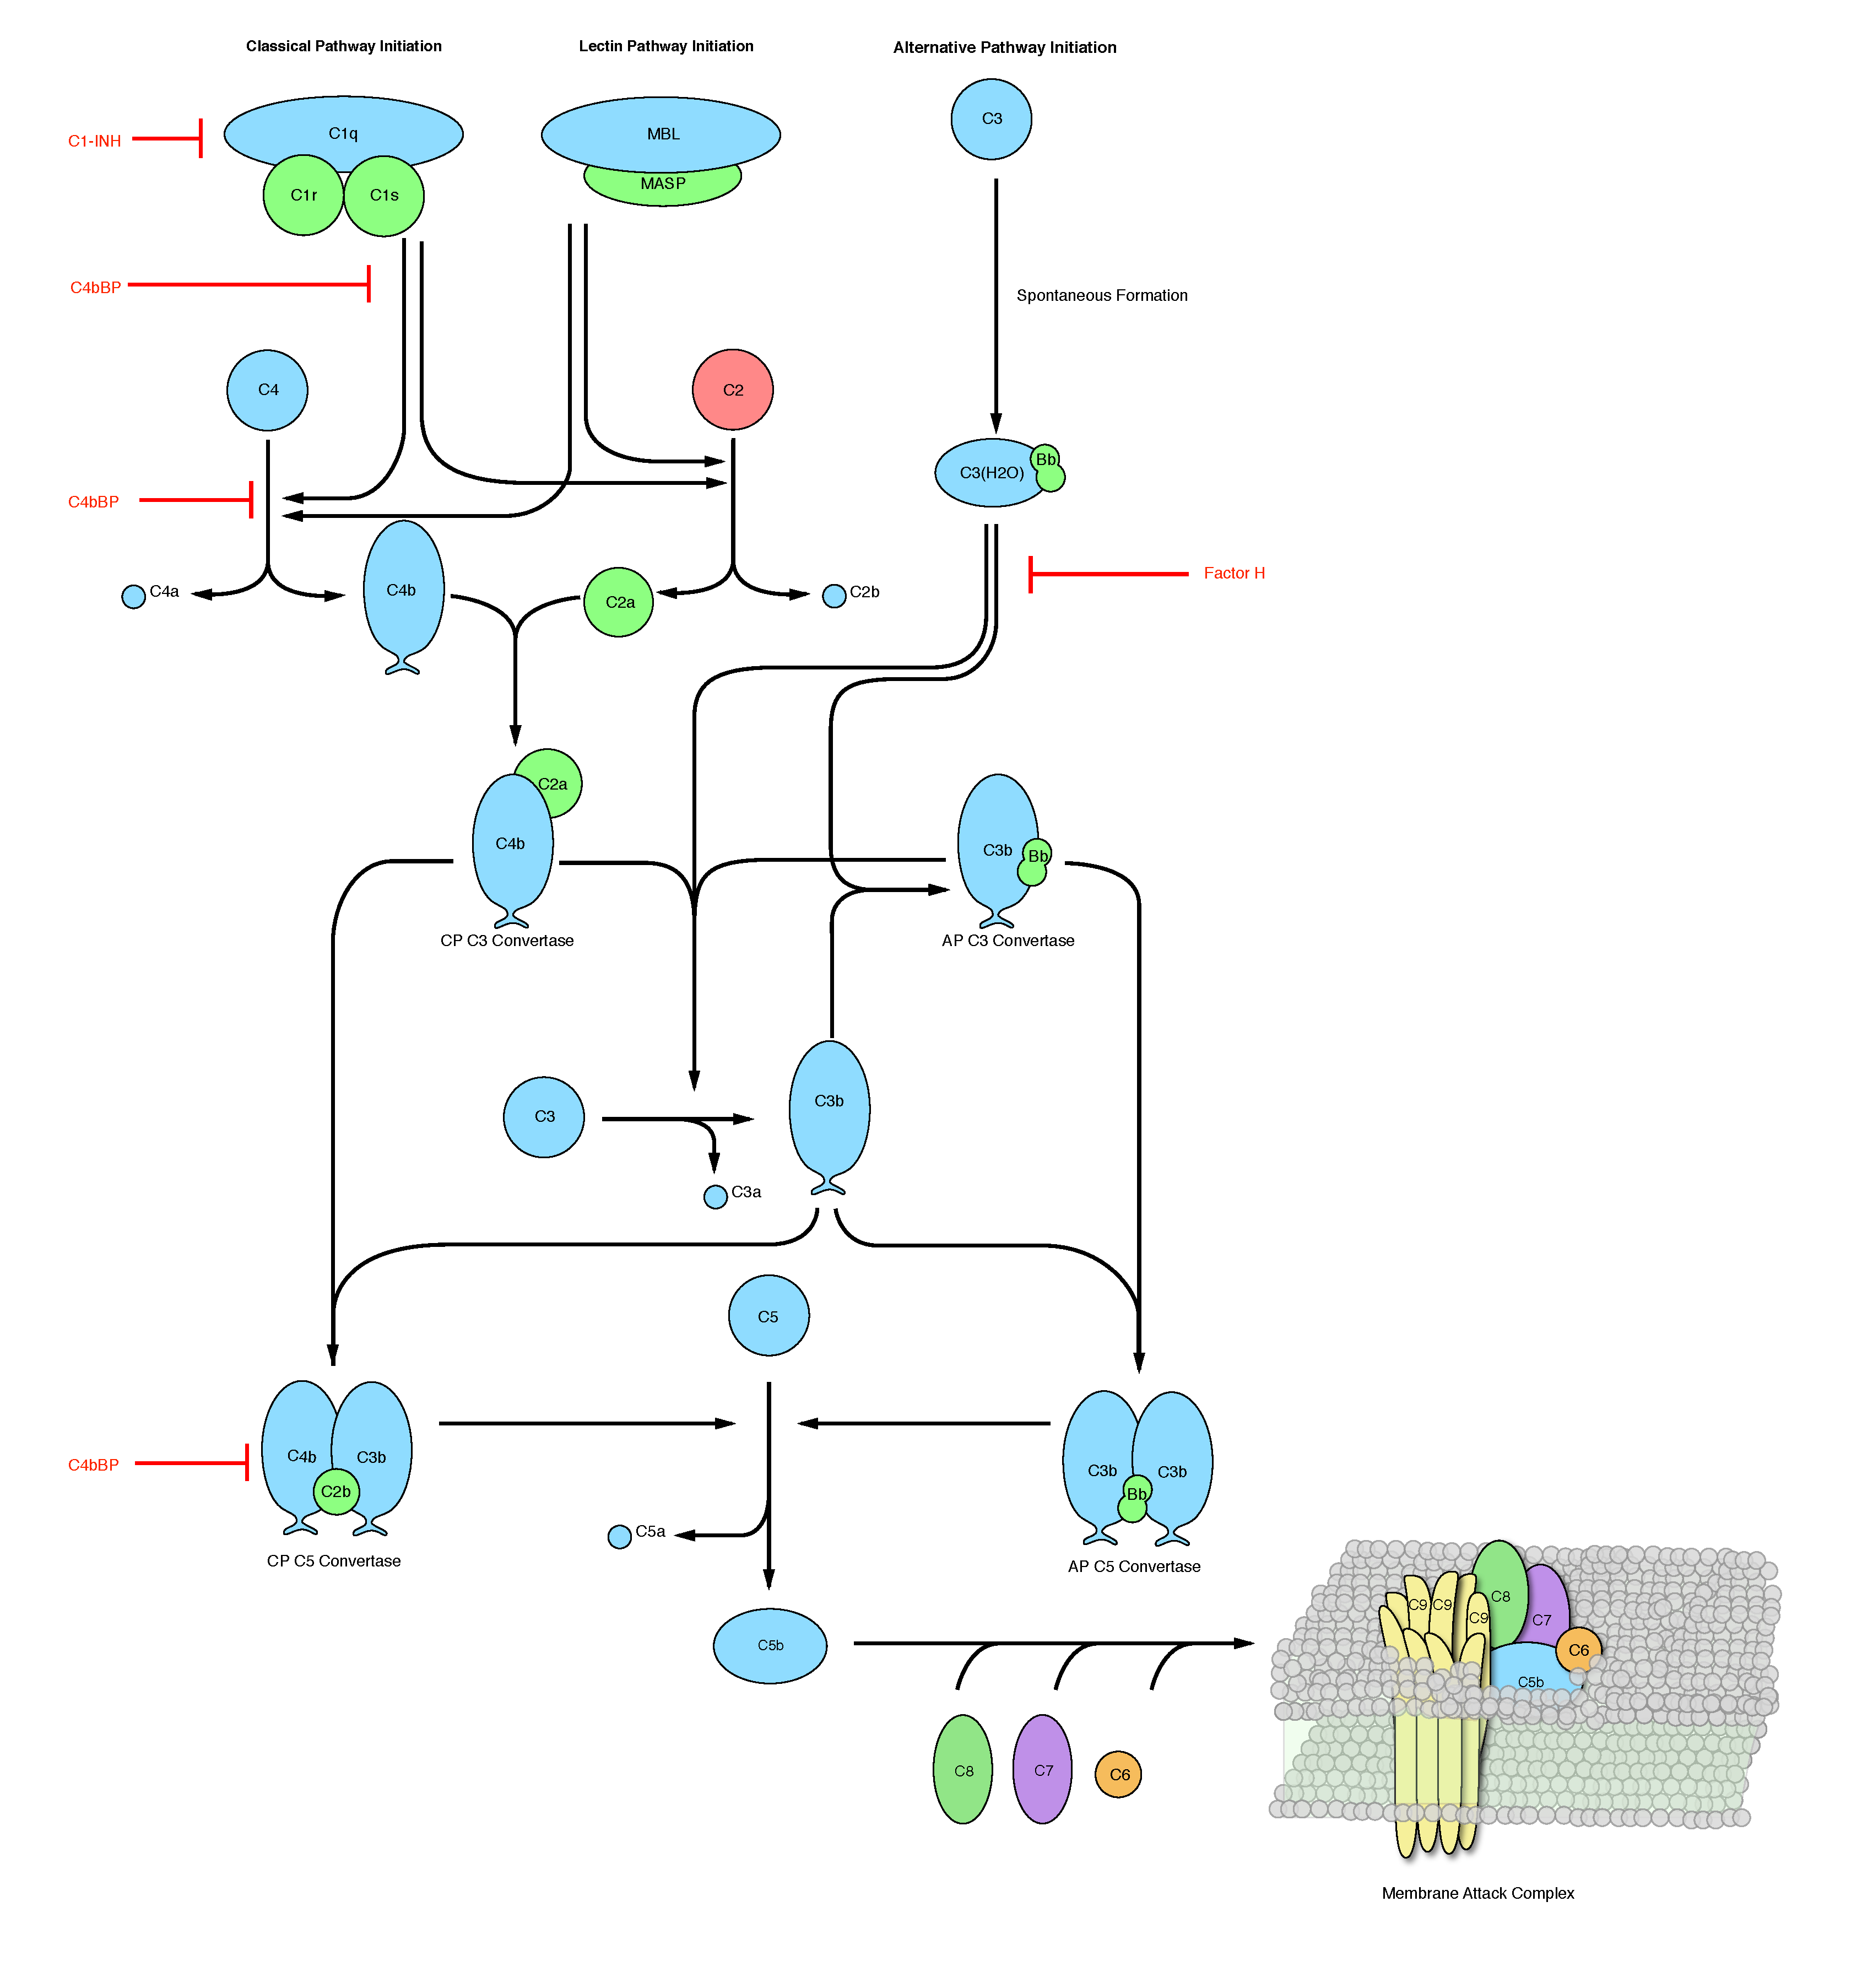
\includegraphics[width=1.0\textwidth]{./figs/ComplementSystemSchematic_v2.pdf}
\caption{Simplified schematic representation of the human complement system. The complement cascade is activated through any one, or more, of the three pathways: classical, lectin, and alternate pathway. The classical pathway is activated by the complex formation of $C1q$, $C1r$, and $C1s$ by the recogniztion of antibody:antigen complexes. Similarly, the lecin pathway is initiation by binding mannan-binding lectin to mannose on pathogen surfaces. Lastly, the alternative pathway is activated when a complement component is spontaneously bound to the surface of the pathogen of virus. The activation from the three pathways creates a cascades of reactions that forms the proteases, $C3$ Convertase that cleaves $C3$ into $C3a$, and $C3b$, the main effector molecule of the complement system. $C3b$ can find to a $C3$ convertase and form a $C5$ convertase that cleaves $C5$ into $C5a$, and $C5b$ that undergoes a series of reactions to form the membrane attach complex ($MAC$).}\label{fig-schematic}
\end{figure}

\begin{figure}[h]
\centering
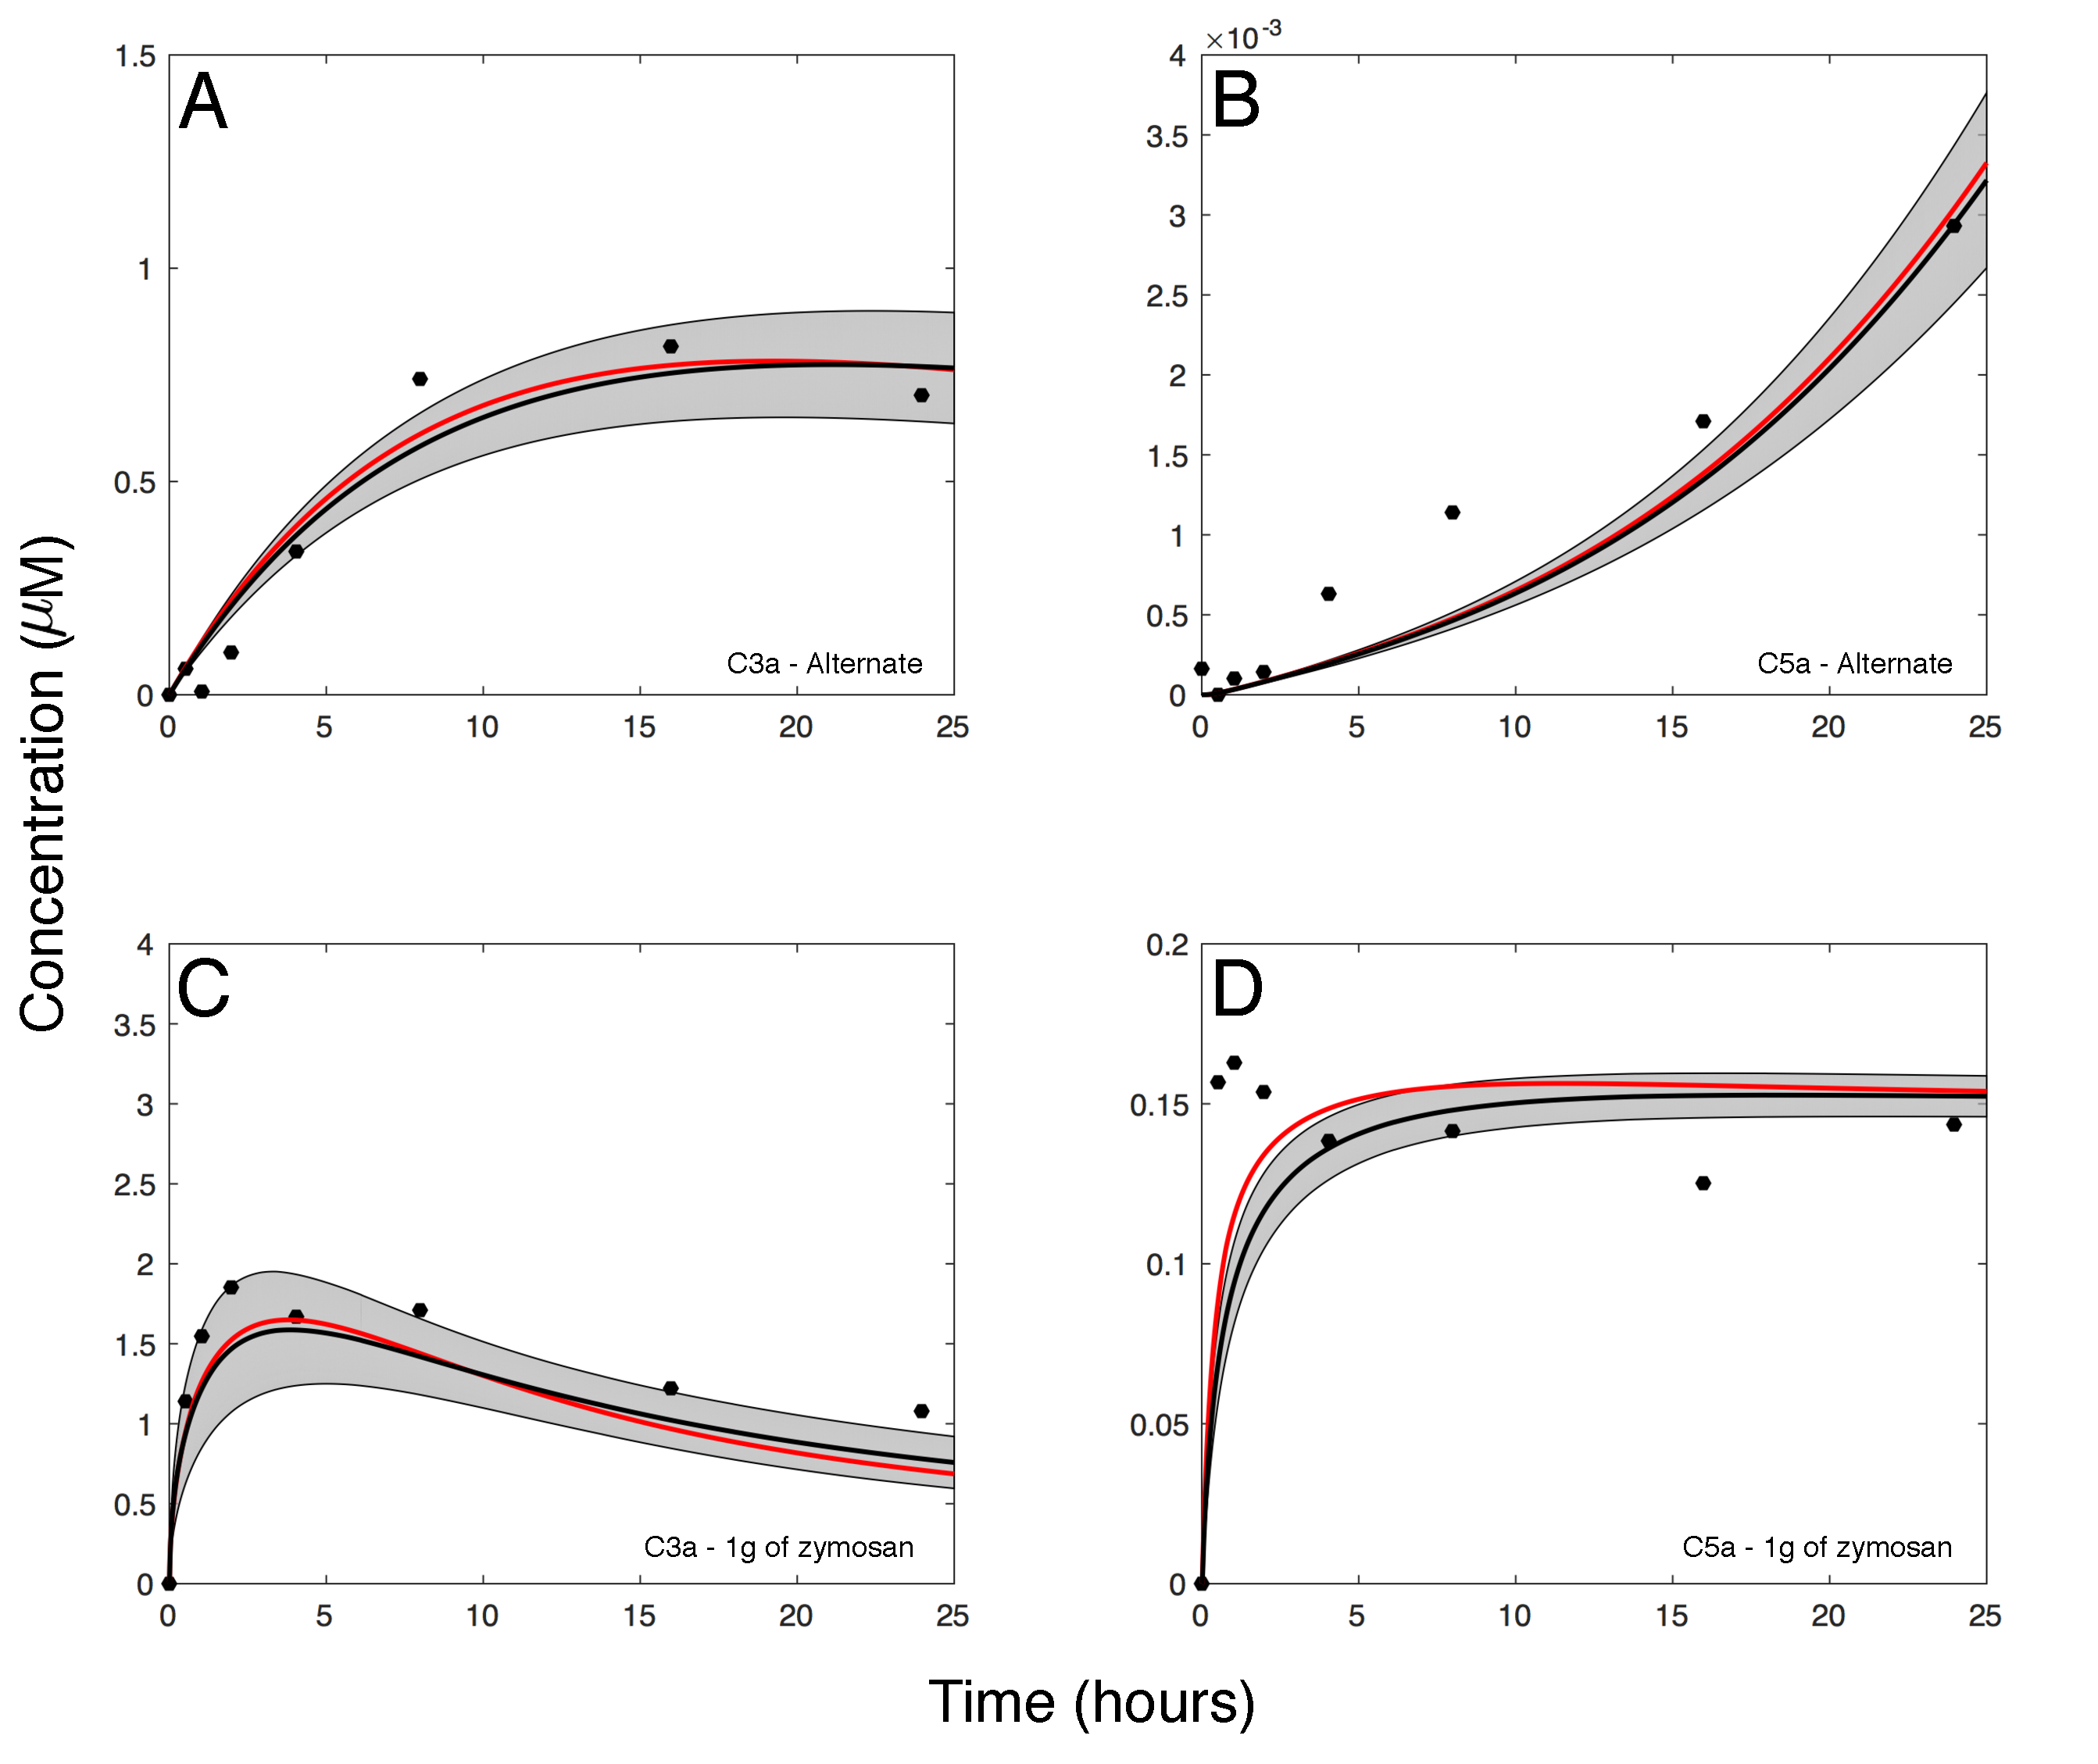
\includegraphics[width=1.0\textwidth]{./figs/Figure2_Fit.pdf}
\caption{Reduced order complement model training simulation for lectin and alternative pathway in presence of zymosan. Reduced order complement model parameters were estimated using Dynamic Optimization with Particle Swarms (DOPS) using the availability of zymosan as a function of lectin pathway initiation.  Only parameters that govern the behavior of alternative pathway were allowed to vary when zymosan was not present. Our model training was conducted in a hierarchal fashion where the alternate parameters were trained and then used and fixed in estimating the lectin parameters. The red line shows the best-fit parameter, the black lines denotes the simulated mean value of $C3a$ or $C5a$ for a 50 parameter set ensemble. The shaded region denotes the distribution of $C3a$ and $C5a$ of the ensemble.}\label{fig-fit}
\end{figure}

\begin{figure}[h]
\centering
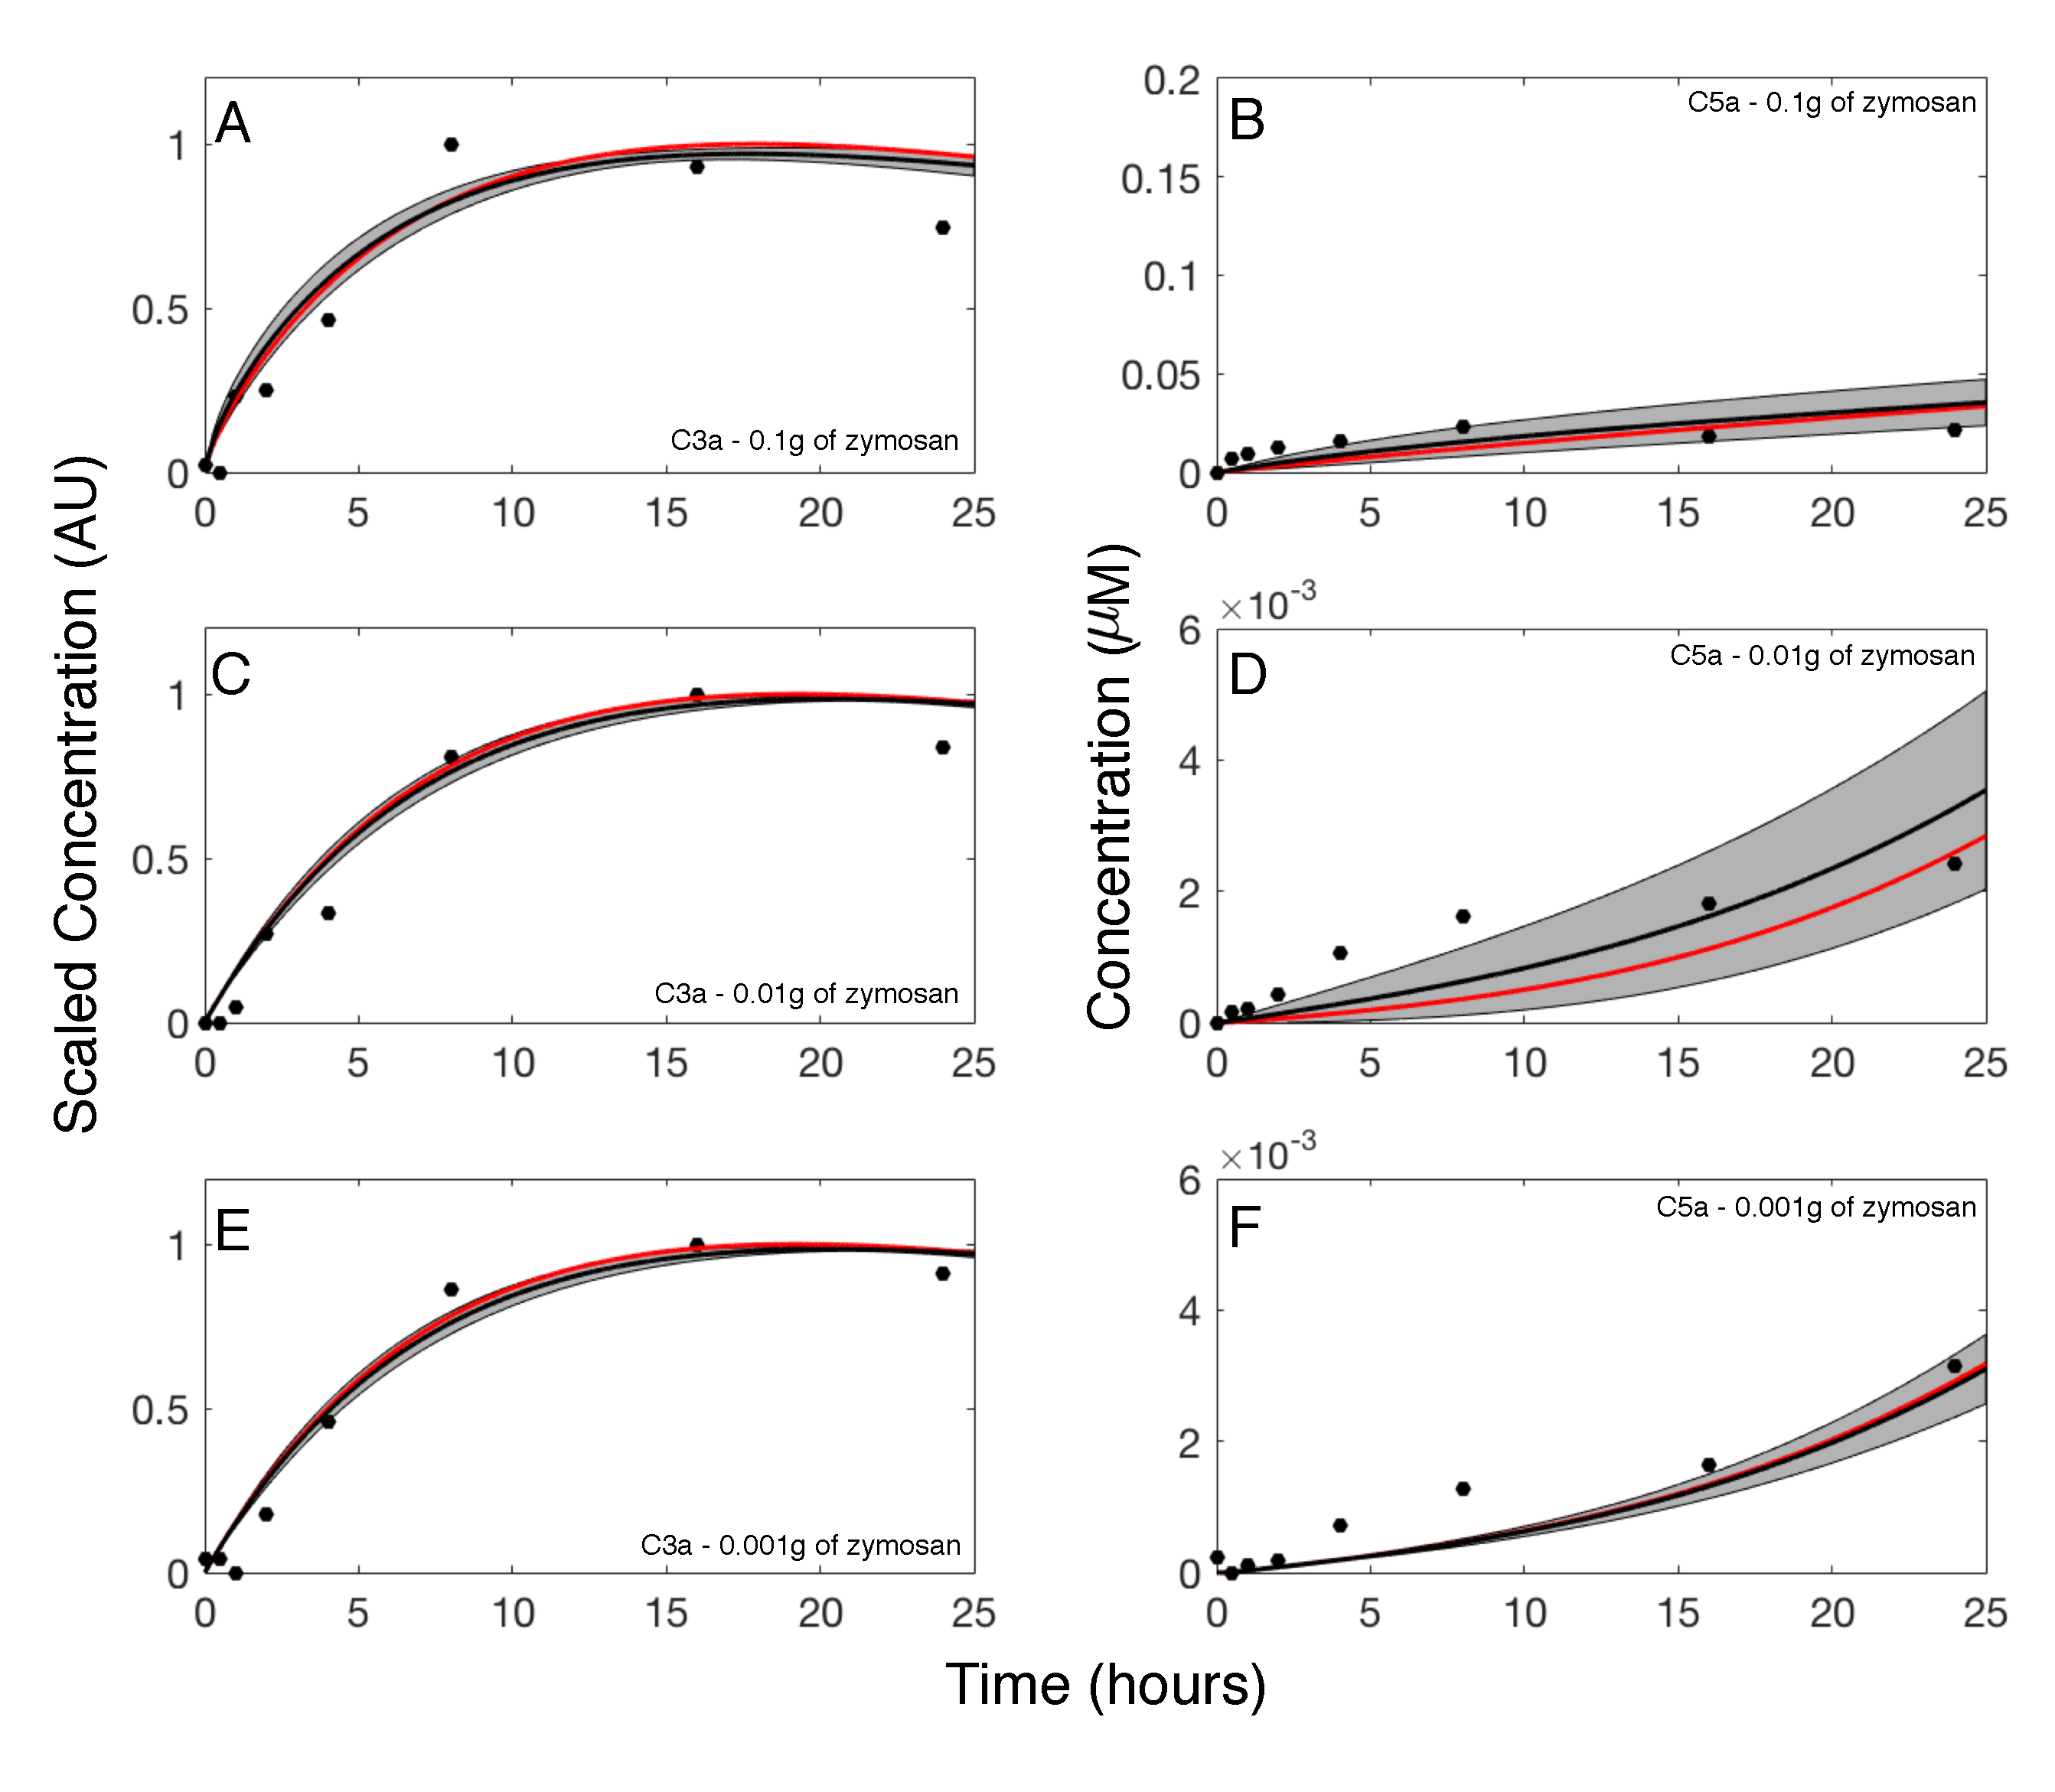
\includegraphics[width=1.0\textwidth]{./figs/Figure3_Predictions_2.pdf}
\caption{Reduced order complement model predictions of lectin and alternative pathway in presence of zymosan. (A-F) Simulation of complement dynamics in the presence of zymosan were conducted for a range of trigger values ($0.1$, $0.01$, and $0.001$ grams of zymosan). The time-course profiles of $C3a$ and $C5a$ under three different zymosan concentrations were simulated using 50 ensembles of trained parameter sets against experimental data of Shaw et al [REF].  The red curve represents the best fit parameter, grey shaded region denotes the prediction results from 50 ensembles of parameter sets, and the black curve is the mean of the ensemble. All complement protein and factor initial concentrations coincided with human serum levels unless otherwise noted.}\label{fig-prediction}
\end{figure}

\begin{figure}[h]
\centering
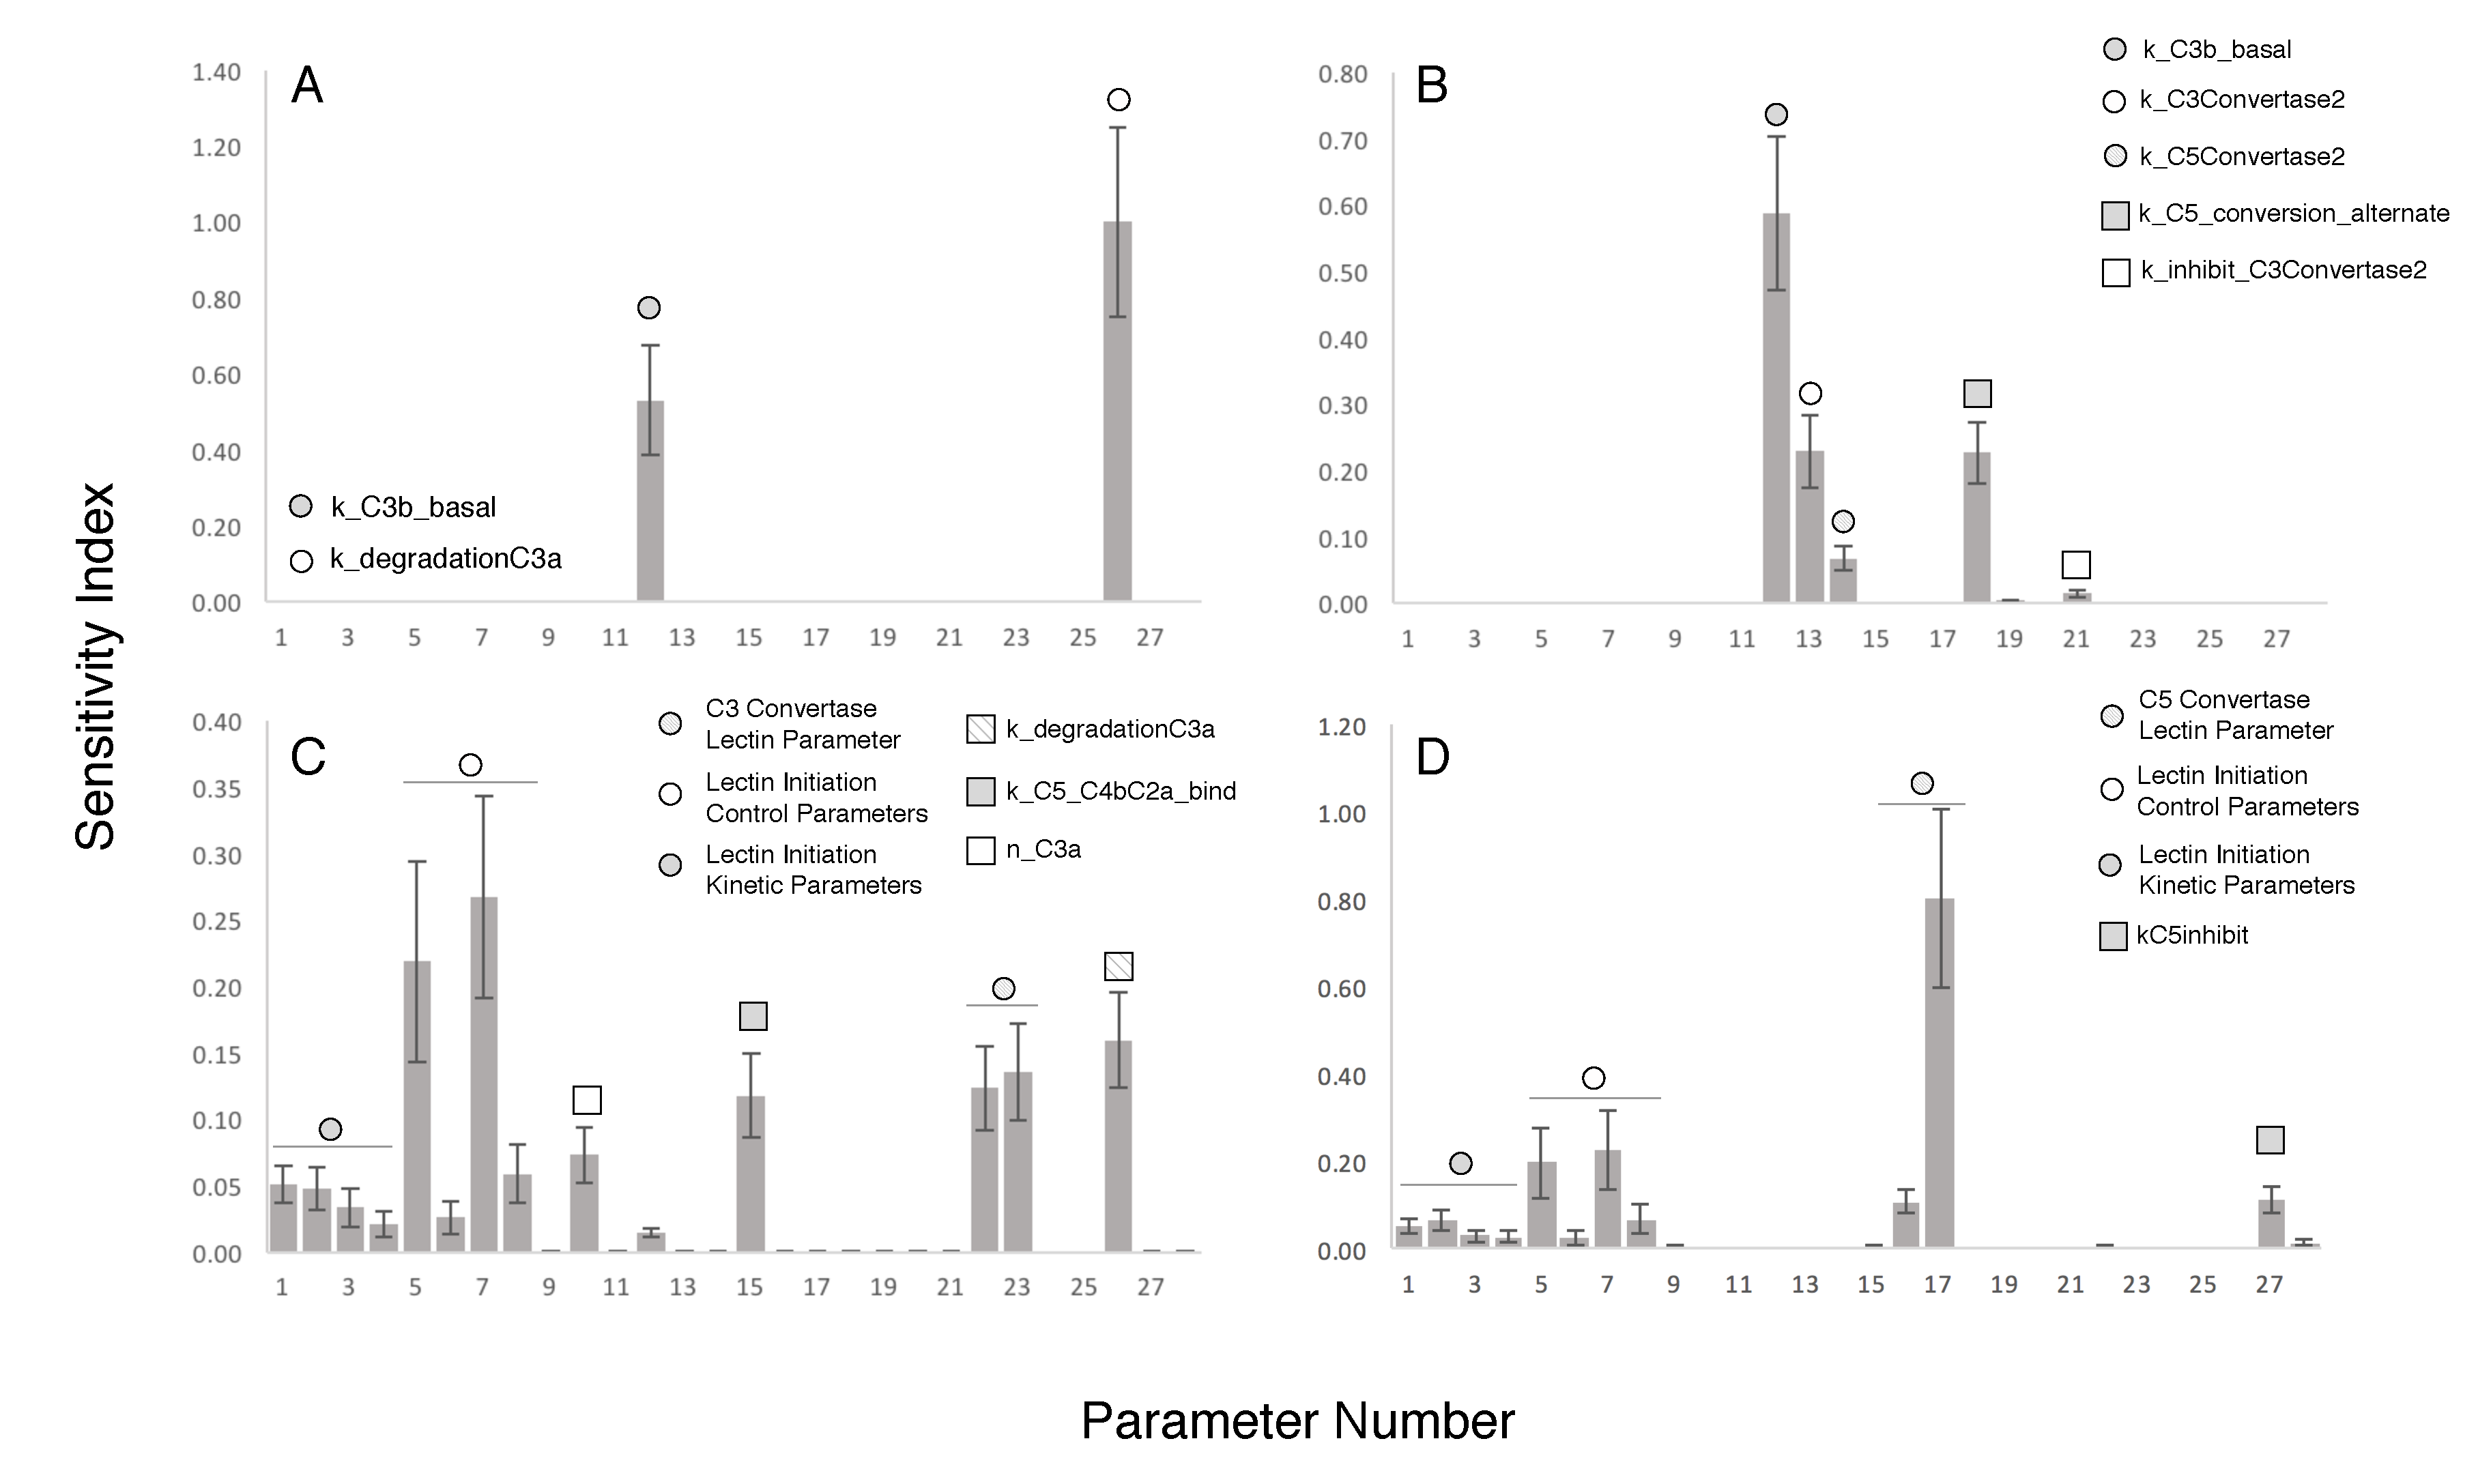
\includegraphics[width=1.0\textwidth]{./figs/Figure4_Sensitivity_Analysis_may24.pdf}
\caption{Sobol's sensitivity analysis of the reduced order complement model with respect to the modeling parameters.  Sensitivity analysis was conducted on the four cases we used to train our model: (A) C3a at 0 zymosan, (B) C5a 0 zymosan, (C) C3a 1 g zymosan, and (D) C5a $1$ g zymosan. The bars denote total sensitivity index which includes local contribution of each parameter and global sensitivity of significant pairwise interactions. The error bars are the 95 percent confidence interval. $k$ represents association rate, $km$ denote Michaelis-Menten saturation constants, and $alpha$ and $n$ refers to the exponentials of the control functions.}\label{fig-SA}
\end{figure}

\clearpage

% Supplemental figures -
% Set the S-
\renewcommand\thefigure{S\arabic{figure}}
\renewcommand\thetable{T\arabic{table}}
\renewcommand\thepage{S-\arabic{page}}
\renewcommand\theequation{S\arabic{equation}}

% Reset the counters -
\setcounter{equation}{0}
\setcounter{table}{0}
\setcounter{figure}{0}
\setcounter{page}{1}


\section*{Supplemental materials.}
\subsection*{Model equations.}
The reduced-order complement model consisted of 18 ordinary differential equations, 12 rate equations, and two control equations:
\begin{eqnarray}
	\frac{dx_{1}}{dt} & =& - r_{1}f_{1} \\ 								%C4
	\frac{dx_{2}}{dt} &=& - r_{2}f_{2} \\  								%C2
	\frac{dx_{3}}{dt} &=&  r_{1}f_{1} \\ 								%C4a
	\frac{dx_{4}}{dt} &=& r_{1}f_{1} - r_{6} \\ 					%C4b
	\frac{dx_{5}}{dt} & = & r_{2}f_{2} - r_{6} \\ 					%C2a
	\frac{dx_{6}}{dt} &=& r_{2}f_{2} \\ 								%C2b
	\frac{dx_{7}}{dt} &=& r_{3} - r_{4} - r_{5}\\ 				%C3
	\frac{dx_{8}}{dt} &=& r_{3}  + r_{4} + r_{5}  - k_{deg,c3a}*C3a \\		%C3a
	\frac{dx_{9}}{dt} &=& r_{3}  + r_{4} + r_{5}  -  r_{7} \\		%C3b
	\frac{dx_{10}}{dt} &=& r_{6} - r_{10} -  r_{8} \\			%CP C3C
	\frac{dx_{11}}{dt} &=& r_{7} - r_{11} -  r_{9} \\			%AP C3C
	\frac{dx_{12}}{dt} &=& r_{10} - r_{14} \\							%CP C5C
	\frac{dx_{13}}{dt} &=& r_{10}  \\											%AP C5C
	\frac{dx_{14}}{dt} &=& - r_{12} - r_{13} \\								%C5
	\frac{dx_{15}}{dt} &=&  r_{12} + r_{13} - k_{deg,c5a} \\					%C5a
	\frac{dx_{16}}{dt} &=& r_{12} + r_{13} \\								%C5b
	\frac{dx_{17}}{dt} &=& - r_{8} - r_{14} \\  				         %C4BP
	\frac{dx_{18}}{dt} &=& - r_{9} \\									%Factor H
\end{eqnarray}where the rate equations are given by:
\begin{eqnarray}
	r_{1} &=& \frac{k_{i1}(C4)}{(K_{1s} + C4)} \\
	r_{2} &=& \frac{k_{2}(C2)}{(K_{2s} + C2)} \\
	f_{1} &=& \frac{Zymo^{\eta_{1}}}{(Zymo^{\eta_{1}} + \alpha_{1}^{\eta_{1}})} \\
	f_{2} &=& \frac{Zymo^{\eta_{2}}}{(Zymo^{\eta_{2}} + \alpha_{2}^{\eta_{2}})} \\
	r_{3} &=& k_{3}(C3) \\
	r_{4} &=& \frac{k_{4}(C3C_{L})(C3^{\eta_{3})}}{(K_{4s}^{\eta_{3}} + C3^{\eta_{3}})}  \\
	r_{5} &=& \frac{k_{5}(C3C_{A})(C3)}{(K_{5s} + C3)} \\
	r_{6} &=& k_{6}(C4b)(C2a) \\
	r_{7} &=& k_{7}(C4b)(C2a) \\
	r_{8} &=& k_{8}(C3C_{L})(C4b)(C4BP) \\
	r_{9} &=& k_{9}(C3C_{A})(FactorH) \\
	r_{10} &=& k_{10}(C3C_{L})(C3b) \\
	r_{11} &=& k_{11}(C3C_{A})(C3b) \\
	r_{12} &=& \frac{k_{12}(C5C_{L})(C5^{\eta_{4}})}{(K_{12s}^{\eta_{4}} + C5^{\eta_{4}})} \\
	r_{13} &=& \frac{k_{13}(C5C_{A})(C5)}{(K_{13s} + C5)} \\
	r_{14} &=& k_{14}(C5C_{L})(C4BP)
\end{eqnarray}

% Supplemental figures go here ...
%\begin{figure}[ht]
%\centering
%\includegraphics[width=1.00\textwidth]{./figs/<Filename>.pdf}
%\caption{Captiontext goes here}
%}\label{fig:<label_name>}
%\end{figure}

\end{document}
